\chapter{Perancangan}
\label{chap:perancangan}

Bab ini membahas tentang perancangan setiap fitur yang akan diimplementasi pada perangkat lunak \textit{Sharif Judge}. 

\section{Mengganti method \textit{shell\_exec("rm ...")} menjadi \textit{unlink()}}
\textit{Method} \textit{shell\_exec("rm ...")} yang memiliki fungsi untuk menghapus sebuah file terdapat pada file \textit{controller Assignment.php} tepatnya di baris kode 425 dan 473

\textit{Assignments.php}
\begin{lstlisting}[basicstyle=\ttfamily, frame=single,
columns=fullflexible, keepspaces=true]

...
423	// Upload Tests (zip file)
424	
425	shell_exec('rm -f '.$assignments_root.'/*.zip');
426	$config = array(
...
472	foreach($old_pdf_files as $old_name)
473		shell_exec("rm -f $old_name");
474	$this->messages[] = array(
...

\end{lstlisting}

Fungsi \textit{shell\_exec("rm ...")} pada baris 425 dan 473 akan diubah menggunakan fungsi \textit{unlink()} menjadi seperti berikut

\textit{Assignments.php}
\begin{lstlisting}[basicstyle=\ttfamily, frame=single,
columns=fullflexible, keepspaces=true]

...
423	// Upload Tests (zip file)
424	
425	unlink($assignments_root.'/*.zip');
426	$config = array(
...
472	foreach($old_pdf_files as $old_name)
473		unlink($old_name);
474	$this->messages[] = array(
...

\end{lstlisting}

\section{Menambahkan method rekoneksi ke \textit{database}}
\textit{Method} rekoneksi ke \textit{database} akan ditambahkan pada \textit{file controller Queueprocess.php}. 

\textit{Queueprocess.php}
\begin{lstlisting}[basicstyle=\ttfamily, frame=single,
columns=fullflexible, keepspaces=true]

...
133
134	// Save the result
135	$this->queue_model->save_judge_result_in_db($submission, $type);
...

\end{lstlisting}

\textit{Method} rekoneksi yang digunakan yaitu \textit{\$this->db->reconnect()}. \textit{Method} ini diletakan pada baris 134 tepat sebelum \textit{Sharif Judge} menyimpan hasil \textit{judge}. Hal tersebut dilakukan untuk menghindari \textit{connection times out} akibat pengujian yang memakan waktu lama.

\textit{Queueprocess.php}
\begin{lstlisting}[basicstyle=\ttfamily, frame=single,
columns=fullflexible, keepspaces=true]

...
133
134	//reconnect to database incase we have run test for a long time.
135	$this->db->reconnect();
136
137	// Save the result
138	$this->queue_model->save_judge_result_in_db($submission, $type);
...

\end{lstlisting}

\section{Membatasi soal (deskripsi \& PDF) hanya bisa diunduh saat \textit{assignment "open"} dan setelah waktu mulai}
Fungsi untuk mengunduh soal (deskripsi \& PDF) terdapat pada \textit{controller Assignment.php} tepatnya di baris kode 100.

\textit{Assignments.php}
\begin{lstlisting}[basicstyle=\ttfamily, frame=single,
columns=fullflexible, keepspaces=true, breaklines=true]

97	/**
98	* Download pdf file of an assignment (or problem) to browser
99	*/
100	public function pdf($assignment_id, $problem_id = NULL)
101	{
102		// Find pdf file
103		if ($problem_id === NULL)
104			$pattern = rtrim($this->settings_model->get_setting('assignments_root'),'/')."/assignment_{$assignment_id}/*.pdf";
105		else
106			$pattern = rtrim($this->settings_model->get_setting('assignments_root'),'/')."/assignment_{$assignment_id}/p{$problem_id}/*.pdf";
107		$pdf_files = glob($pattern);
108		if ( ! $pdf_files )
109			show_error("File not found");
110
111		// Download the file to browser
112		$this->load->helper('download')->helper('file');
113		$filename = shj_basename($pdf_files[0]);
114		force_download($filename, file_get_contents($pdf_files[0]), TRUE);
115	}

\end{lstlisting}

Selain membatasi soal (deskripsi \& PDF) hanya dapat diunduh saat \textit{assignment "open"} dan setelah waktu mulai, pada fungsi ini juga ditambahkan fitur lain. Fitur lain tersebut yaitu membatasi soal hanya dapat diunduh oleh peserta yang terdaftar sebagai "\textit{participant}" dan soal tidak dapat diunduh setelah melewati batas waktu pengumpulan. Rancangan algoritma kode yang akan digunakan yaitu
\begin{itemize}
	\item Membuat atribut tambahan untuk menyimpan informasi waktu selesai, waktu mulai dan waktu tambahan sebuah assignment.
	\item Jika atribut "\textit{open}" pada \textit{assignment} tidak memiliki nilai, maka munculkan pesan \textit{error} "\textit{Selected assignment has been closed}."
	\item Jika pengguna tidak terdaftar sebagai "\textit{participant}" dalam \textit{assignment} yang dipilih, maka munculkan pesan error "\textit{You are not registered for submitting}."
	\item Jika waktu sekarang telah melewati batas waktu selesai + waktu tambahan, maka munculkan pesan \textit{error} "\textit{Selected assignment has finished}."
	\item Jika waktu sekarang belum melewati waktu mulai, maka munculkan pesan \textit{error} "\textit{Selected assignment has not started}."	
\end{itemize}

Berikut hasil pengimplementasian rancangan algoritma di atas ke dalam kode program

\textit{Assignments.php}
\begin{lstlisting}[basicstyle=\ttfamily, frame=single,
columns=fullflexible, keepspaces=true, breaklines=true]

...
97	/**
98	* Download pdf file of an assignment (or problem) to browser
99	*/
100	public function pdf($assignment_id, $problem_id = NULL)
101	{
102		$finishtime = strtotime($this->assignment_model->assignment_info($assignment_id)['finish_time']);
103		$starttime = strtotime($this->assignment_model->assignment_info($assignment_id)['start_time']);
104		$extratime = $this->assignment_model->assignment_info($assignment_id)['extra_time'];
105
106		// Find pdf file
107		if ($problem_id === NULL)
108			$pattern = rtrim($this->settings_model->get_setting('assignments_root'),'/')."/assignment_{$assignment_id}/*.pdf";
109		else
110			$pattern = rtrim($this->settings_model->get_setting('assignments_root'),'/')."/assignment_{$assignment_id}/p{$problem_id}/*.pdf";
111		$pdf_files = glob($pattern);
112		if ( ! $pdf_files )
113			show_error("File not found");
114		elseif (!$this->assignment_model->assignment_info($assignment_id)['open'])
115			show_error('Selected assignment has been closed.');
116		elseif	( ! $this->assignment_model->is_participant($this->assignment_model->assignment_info($assignment_id)['participants'],$this->user->username) )
117			show_error('You are not registered for submitting.');
118		elseif ( shj_now() > $finishtime + $extratime)
119			show_error('Selected assignment has finished.');
120		elseif ( shj_now() < $starttime)
121			show_error('Selected assignment has not started.');
122			
123		// Download the file to browser
124		$this->load->helper('download')->helper('file');
125		$filename = shj_basename($pdf_files[0]);
126		force_download($filename, file_get_contents($pdf_files[0]), TRUE);
127	}
...

\end{lstlisting}

\section{Mensupport \textit{file} dengan ekstensi TXT}
Untuk dapat mensupport \textit{file} dengan ekstensi TXT pada perangkat lunak \textit{Sharif Judge}, diperlukan penambahan dan perubahan kode pada beberapa \textit{file}. Beberapa \textit{file} tersebut antara lain \textit{controller Submit.php, model Assignment\_model.php, view submissions.twig} dan \textit{file} bantuan \textit{shj\_helper.php} yang terdapat pada direktori \path{Sharif-Judge\helpers\}. Berikut beberapa baris potongan kode program

\textit{Submit.php}
\begin{lstlisting}[basicstyle=\ttfamily, frame=single,
columns=fullflexible, keepspaces=true, breaklines=true]

...
58		case 'java': return 'java';
59		case 'zip': return 'zip';
60		case 'pdf': return 'pdf';
61		default: return FALSE;
62	}
...
76		case 'java': return ($extension==='java'?TRUE:FALSE);
77		case 'zip': return ($extension==='zip'?TRUE:FALSE);
78		case 'pdf': return ($extension==='pdf'?TRUE:FALSE);
79	}
...
88	if ($str=='0')
89		return FALSE;
90	if (in_array( strtolower($str),array('c', 'c++', 'python 2', 'python 3', 'java', 'zip', 'pdf')))
91		return TRUE;
92	return FALSE;
...

\end{lstlisting}

\textit{Assignment\_model.php}
\begin{lstlisting}[basicstyle=\ttfamily, frame=single,
columns=fullflexible, keepspaces=true, breaklines=true]

...
100	$item2 = strtolower($item);
101	if ( ! in_array($item2, array('c','c++','python 2','python 3','java','zip','pdf')))
102		continue;
...

\end{lstlisting}

\textit{shj\_helper.php}
\begin{lstlisting}[basicstyle=\ttfamily, frame=single,
columns=fullflexible, keepspaces=true, breaklines=true]

...
81	case 'java': return 'java';
82	case 'zip': return 'zip';
83	case 'pdf': return 'pdf';
84	default: return FALSE;
...
104	case 'java': return 'Java';
105	case 'zip': return 'Zip';
106	case 'pdf': return 'PDF';
107	default: return FALSE;
...

\end{lstlisting}

\textit{submissions.twig}
\begin{lstlisting}[basicstyle=\ttfamily, frame=single,
columns=fullflexible, keepspaces=true, breaklines=true]

...
160	<td>
161		
162			<div class="btn shj-orange" data-type="download">Download</div>
163		
164			<div class="btn shj-orange" data-type="code" >Code</div>
165		
166	</td>
...

\end{lstlisting}

Penambahan dan perubahan kode dilakukan setelah baris 60, 78 dan 90 pada \textit{controller Submit.php}. Berikut hasil penambahan dan perubahan kode 

\textit{Submit.php}
\begin{lstlisting}[basicstyle=\ttfamily, frame=single,
columns=fullflexible, keepspaces=true, breaklines=true]

...
58		case 'java': return 'java';
59		case 'zip': return 'zip';
60		case 'pdf': return 'pdf';
61		case 'txt': return 'txt';
62		default: return FALSE;
63	}
...
77		case 'java': return ($extension==='java'?TRUE:FALSE);
78		case 'zip': return ($extension==='zip'?TRUE:FALSE);
79		case 'pdf': return ($extension==='pdf'?TRUE:FALSE);
80		case 'txt': return ($extension==='txt'?TRUE:FALSE);
81	}
...
90	if ($str=='0')
91		return FALSE;
92	if (in_array( strtolower($str),array('c', 'c++', 'python 2', 'python 3', 'java', 'zip', 'pdf', 'txt')))
93		return TRUE;
94	return FALSE;
...

\end{lstlisting}

Perubahan kode dilakukan di baris 101 pada model \textit{Assignment\_model.php}. Berikut hasil perubahan kode 

\textit{Assignment\_model.php}
\begin{lstlisting}[basicstyle=\ttfamily, frame=single,
columns=fullflexible, keepspaces=true, breaklines=true]

...
100	$item2 = strtolower($item);
101	if ( ! in_array($item2, array('c','c++','python 2','python 3','java','zip','pdf','txt')))
102		continue;
...

\end{lstlisting}

Penambahan kode dilakukan setelah baris 83 pada \textit{file} bantuan \textit{shj\_helper.php}. Berikut hasil penambahan kode 

\textit{shj\_helper.php}
\begin{lstlisting}[basicstyle=\ttfamily, frame=single,
columns=fullflexible, keepspaces=true, breaklines=true]

...
81	case 'java': return 'java';
82	case 'zip': return 'zip';
83	case 'pdf': return 'pdf';
84	case 'txt': return 'txt';
85	default: return FALSE;
...
105	case 'java': return 'Java';
106	case 'zip': return 'Zip';
107	case 'pdf': return 'PDF';
108	case 'txt': return 'TXT';
109	default: return FALSE;
...

\end{lstlisting}

Perubahan kode dilakukan pada baris 161 pada \textit{view submissions.twig}. Berikut hasil perubahan kode

\textit{submissions.twig}
\begin{lstlisting}[basicstyle=\ttfamily, frame=single,
columns=fullflexible, keepspaces=true, breaklines=true]

...
160	<td>
161		
162			<div class="btn shj-orange" data-type="download">Download</div>
163		
164			<div class="btn shj-orange" data-type="code" >Code</div>
165		
166	</td>
...

\end{lstlisting}

\section{Membuat halaman \textit{Logs} yang mencatat aktivitas \textit{login} pengguna}
Agar halaman \textit{Logs} dapat berjalan dengan baik, perlu ditambahkan tabel baru pada \textit{database} \textit{Sharif Judge}.  \textit{Tabel} baru tersebut akan bernama \textit{shj\_logins}. 
\begin{table}[H] %atau h saja untuk "kira kira di sini"
	\centering 
	\caption{Perancangan Tabel \textit{shj\_logins}}
	\label{tab:tabellogs}
		\begin{tabular}{|c|c|c|c|}
			\hline
			\textbf{Atribut} & \textbf{Tipe Data} & \textbf{Ukuran}  & \textbf{Default} \\
			\hline
			\textit{login\_id} (PK*) & int & 11  & None \\
			\hline
			\textit{username} & varchar & 20  & None \\
			\hline
			\textit{ip\_address} & varchar & 15  & None \\
			\hline
			\textit{timestamp} & timestamp & 11  & current\_timestamp \\
			\hline
			\textit{last\_24h\_login\_id}	 & int & 11  & null \\
			\hline
		\end{tabular}
\end{table}
*PK = \textit{Primary Key}.

Keterangan atribut:
\begin{enumerate}
	\item \textit{login\_id}: sebagai penanda yang membedakan setiap \textit{login} peserta satu dengan yang lain. Memiliki \textit{length default} int dari \textit{phpMyAdmin} yaitu 11. Atribut \textit{login\_id} merupakan \textit{primary key} karena id harus unik agar setiap \textit{login} peserta dapat dibedakan. Atribut ini juga bersifat \textit{auto increment}.
	\item \textit{username}: \textit{username} peserta yang berhasil \textit{login} pada \textit{Sharif Judge}. Memiliki \textit{length varchar} 20 karena \textit{length username} pada tabel \textit{shj\_users} adalah 20.
	\item \textit{ip\_address}: \textit{ip address} peserta yang berhasil \textit{login} pada \textit{Sharif Judge}. Memiliki \textit{length varchar} 15 karena \textit{length} maksimal dari \textit{ip address protocol version 4 (IPv4)} adalah 15. Contoh: 202.100.123.255
	\item \textit{timestamp}: waktu peserta saat berhasil \textit{login} pada \textit{Sharif Judge}. Menggunakan tipe data timestamp yang akan mencatat waktu \textit{login} dengan format YYYY-MM-DD HH:MM:SS. Contoh: 2018-04-06 18:15:43
	\item \textit{last\_24h\_login\_id}: id \textit{login} peserta yang berhasil \textit{login} pada \textit{Sharif Judge} namun menggunakan \textit{ip address} berbeda dalam waktu 24 jam terakhir.
\end{enumerate}

Selain tabel diatas, halaman logs juga akan ditambahkan \textit{model, view} dan \textit{controller}.
\begin{enumerate}
	\item \textit{Model} \\
	\textit{Model} untuk halaman \textit{logs} akan bernama \textit{Logs\_model.php}. Berikut adalah perincian fungsi yang terdapat dalam rancangan \textit{model Logs\_model.php}.
	\begin{table}[H]
		\caption{Perincian fungsi \textit{insert\_to\_logs}}
		\begin{tabular}{|c|p{11cm}|}
			\hline
			Nama \textit{Method} 	& 	\textit{insert\_to\_logs} 	\\
			\hline
			Parameter \textit{Input} & \textit{\$username} dan \textit{\$ip\_address} \\
			\hline
			Parameter \textit{Output} & -\\
			\hline
			Tabel yang berhubungan & \textit{shj\_logins} \\
			\hline
			Deskripsi	& Proses untuk memasukan \textit{logs} pengguna \textit{Sharif Judge} \\
			\hline
			Algoritma	& \begin{itemize}
				\item mengecek dan menghapus \textit{logs} pada tabel \textit{shj\_logins} yang \textit{timestampnya} lebih dari 24 jam
				\item mengecek entri \textit{login} terakhir untuk \textit{\$username} yang  menggunakan \textit{IP address} tidak sama dengan \textit{\$ip\_address}
				\item jika tidak memiliki hasil, maka tambahkan entri baru menggunakan \textit{\$username} dan \textit{\$ip\_address} tersebut
				\item jika memiliki hasil,  maka tambahkan entri baru menggunakan \textit{\$username} dan \textit{\$ip\_address} serta last\textit{\_24h\_login\_id} diisi dengan \textit{login\_id} sebelumnya
			\end{itemize} \\
			\hline
		\end{tabular}
	\end{table}

	\begin{table}[H]
		\caption{Perincian fungsi \textit{get\_all\_logs}}
		\begin{tabular}{|c|p{11cm}|}
			\hline
			Nama \textit{Method} 	& 	\textit{get\_all\_logs} 	\\
			\hline
			Parameter \textit{Input} & - \\
			\hline
			Parameter \textit{Output} &  semua entri logs dari tabel \textit{shj\_logins}\\
			\hline
			Tabel yang berhubungan & \textit{shj\_logins} \\
			\hline
			Deskripsi	& Proses untuk mengembalikan entri \textit{logs} yang terdapat pada tabel \textit{shj\_logins} \\
			\hline
			Algoritma	& \begin{itemize}
				\item mengembalikan seluruh entri logs yang terdapat pada tabel \textit{shj\_logins} dalam bentuk \textit{array}
			\end{itemize} \\
			\hline
		\end{tabular}
	\end{table}

	\item View \\
	\textit{View} untuk halaman \textit{logs} akan bernama \textit{Logs.twig}. Menu halaman \textit{logs} akan terletak di bawah menu \textit{Scoreboard} dan akan bernama '\textit{24-hour log}'. Berikut adalah rancangan tampilan halaman \textit{logs}.
	
	\begin{figure}[H]
		\centering  
		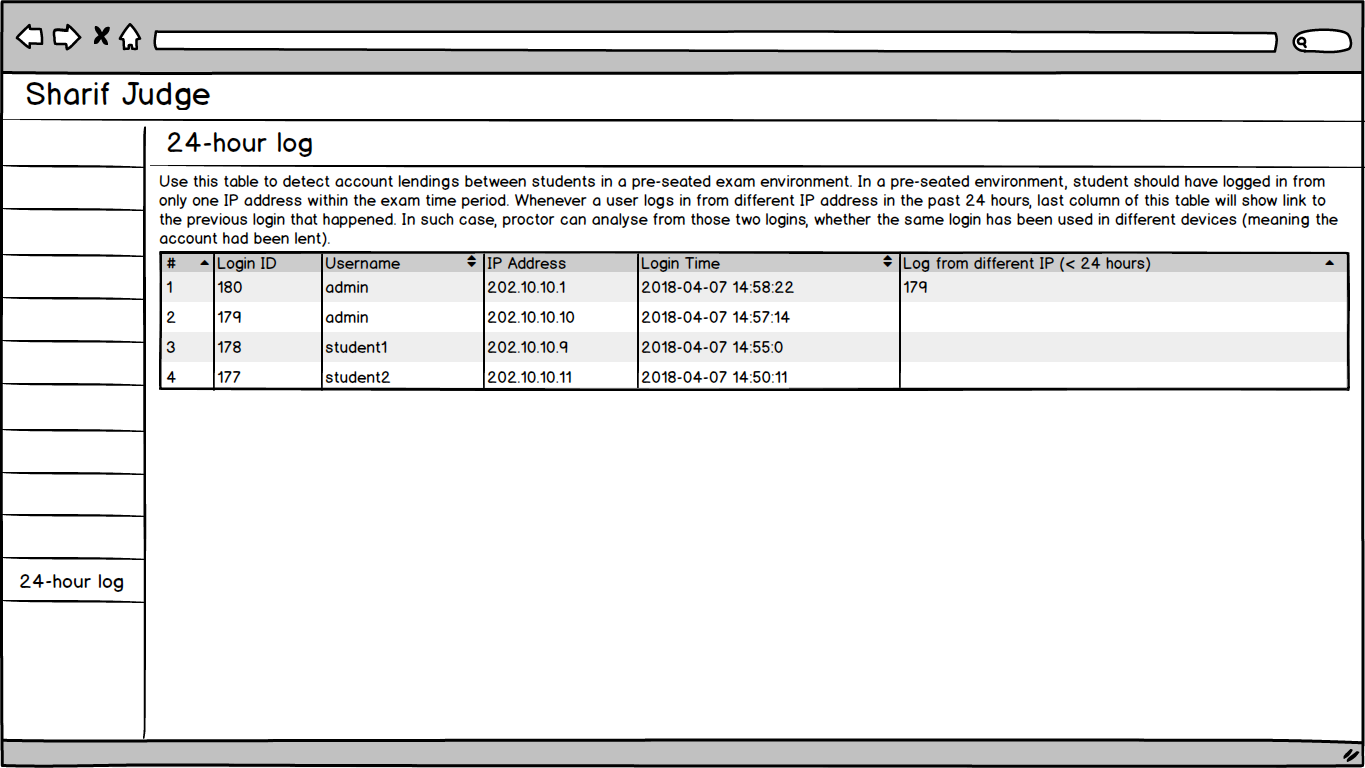
\includegraphics[width=1.0\textwidth]{mockuplogs}  
		\caption[Rancangan tampilan halaman \textit{logs}]{Rancangan tampilan halaman \textit{logs}} 
		\label{fig:mockuplogs} 
	\end{figure}

	\item \textit{Controller} \\
	\textit{Controller} untuk halaman \textit{logs} akan bernama \textit{Logs.php}. Berikut adalah perincian fungsi yang terdapat dalam rancangan \textit{controller Logs.php}.
	\begin{table}[H]
		\caption{Perincian fungsi \textit{consturct\_\_}}
		\begin{tabular}{|c|p{11cm}|}
			\hline
			Nama \textit{Method} 	& 	\textit{consturct\_\_} 	\\
			\hline
			Parameter \textit{Input} & - \\
			\hline
			Parameter \textit{Output} &  - \\
			\hline
			Tabel yang berhubungan & - \\
			\hline
			Deskripsi	& membatasi pengguna yang dapat mengakses halaman \textit{logs}	 \\
			\hline
			Algoritma	& \begin{itemize}
				\item mengecek \textit{session} pengguna yang akan mengakses halaman \textit{logs}
				\item jika \textit{session} tidak berstatus '\textit{logged\_in}, maka pengguna akan dialihkan ke halaman \textit{login}
				\item mengecek \textit{role} pengguna yang akan mengakses halaman \textit{logs}
				\item jika role pengguna bukan \textit{admin}, maka pengguna akan dialihkan ke halaman \textit{'404 Not Found'}
			\end{itemize} \\
			\hline
		\end{tabular}
	\end{table}
	
	\begin{table}[H]
		\caption{Perincian fungsi \textit{index}}
		\begin{tabular}{|c|p{11cm}|}
			\hline
			Nama \textit{Method} 	& 	\textit{index} 	\\
			\hline
			Parameter \textit{Input} & - \\
			\hline
			Parameter \textit{Output} &  - \\
			\hline
			Tabel yang berhubungan & \textit{shj\_logins} \\
			\hline
			Deskripsi	& Proses untuk memuat seluruh entri \textit{logs} pada halaman \textit{Logs.twig}	 \\
			\hline
			Algoritma	& \begin{itemize}
				\item memuat data \textit{logs} menggunakan fungsi \textit{get\_all\_logs} dari \textit{model Logs\_model.php}
				\item memproses data untuk tampilan \textit{Logs.twig}
			\end{itemize} \\
			\hline
		\end{tabular}
	\end{table}
\end{enumerate}

\section{Menambahkan parameter "\textit{Display Name}" pada pendaftaran peserta \textit{Sharif Judge}}
Untuk dapat menambahkan parameter "\textit{Display Name}" pada pendaftaran peserta \textit{Sharif Judge}, diperlukan beberapa perubahan dan penambahan kode. Berikut rancangan algoritma yang akan dilakukan
\begin{enumerate}
	\item Menambahkan parameter "\textit{Display Name}" pada fungsi \textit{add\_user} yang terdapat di \textit{model User\_model.php}.
	\item Mengubah pemisah (\textit{separator}) antar parameter pada fungsi \textit{add\_user}. Pemisah antar parameter yang awalnya menggunakan spasi akan diubah menggunakan tanda koma.
	\item Menambahkan keterangan parameter "\textit{Display Name}" pada halaman \textit{add\_user.twig} dan  \textit{add\_user\_result.twig}.
	\item Menambahkan \textit{Display Name} untuk \textit{admin} pada proses \textit{install Sharif Judge}.
	\item Mengubah urutan data yang digunakan pada fungsi pendaftaran peserta melalui \textit{email}.
	\item Menambahkan \textit{text field Display Name} pada halaman \textit{Register} \textit{(Open Public Registration}).
\end{enumerate}
Dari algoritma yang akan diterapkan, terdapat beberapa perubahan dan penambahan kode pada beberapa \textit{file}. Beberapa file tersebut antara lain \textit{controller Install.php, controller Login.php, model User\_model.php, view add\_user.twig, view add\_user\_result.twig} dan \textit{view register.twig}.
Berikut beberapa baris potongan kode program

\textit{Install.php}
\begin{lstlisting}[basicstyle=\ttfamily, frame=single,
columns=fullflexible, keepspaces=true, breaklines=true]

...
252	// add admin user
253	$this->user_model->add_user(
254		$this->input->post('username'),
255		$this->input->post('email'),
256		$this->input->post('password'),
257		'admin'
	);
...
\end{lstlisting}
~\\
\textit{Login.php}
\begin{lstlisting}[basicstyle=\ttfamily, frame=single,
columns=fullflexible, keepspaces=true, breaklines=true]

...
92	$this->user_model->add_user(
93		$this->input->post('username'),
94		$this->input->post('email'),
95		$this->input->post('password'),
...
\end{lstlisting}
~\\
\textit{User\_model.php}
\begin{lstlisting}[basicstyle=\ttfamily, frame=single,
columns=fullflexible, keepspaces=true, breaklines=true]

...
120	*/
121	public function add_user($username, $email, $password, $role)
122	{
...
138	'username' => $username,
139	'email' => $email,
140	'password' => $this->password_hash->HashPassword($password),
...
176	$parts = preg_split('/\s+/', $line);
177	if (count($parts) != 4)
178		continue; //ignore lines that not contain 4 parts
...
180	if (strtolower(substr($parts[2], 0, 6)) == 'random')
181	{
182		// generate random password
183		$len = trim(substr($parts[2], 6), '[]');
184		if (is_numeric($len)){
185			$this->load->helper('string');
186			$parts[2] = shj_random_password($len);
187		}
188	}
189	
190	$result = $this->add_user($parts[0], $parts[1], $parts[2], $parts[3]);
191	
192	if ($result === TRUE)
193		array_push($users_ok, array($parts[0], $parts[1], $parts[2], $parts[3]));
194	else
195		array_push($users_error, array($parts[0], $parts[1], $parts[2], $parts[3], $result));
...
230	$text = str_replace('{SITE_URL}', base_url(), $text);
231	$text = str_replace('{ROLE}', $user[3], $text);
232	$text = str_replace('{USERNAME}', $user[0], $text);
233	$text = str_replace('{PASSWORD}', htmlspecialchars($user[2]), $text);
234	$text = str_replace('{LOGIN_URL}', base_url(), $text);
...

\end{lstlisting}
~\\
\textit{add\_user.twig}
\begin{lstlisting}[basicstyle=\ttfamily, frame=single,
columns=fullflexible, keepspaces=true, breaklines=true]

...
66	#
67	# USERNAME EMAIL PASSWORD ROLE
68	#
...

\end{lstlisting}
~\\
\textit{add\_user\_result.twig}
\begin{lstlisting}[basicstyle=\ttfamily, frame=single,
columns=fullflexible, keepspaces=true, breaklines=true]

...
9	
10	<li>Usename: {{ item[0] }} Email: {{ item[1] }} Password: <code>{{ item[2] }}</code> Role: {{ item[3] }}</li>
11	
...
17	
18	<li>Usename: {{ item[0] }} Email: {{ item[1] }} Password: <code>{{ item[2] }}</code> Role: {{ item[3] }} ({{ item[4] }})</li>
19	
...
\end{lstlisting}
~\\
\textit{register.twig}
\begin{lstlisting}[basicstyle=\ttfamily, frame=single,
columns=fullflexible, keepspaces=true, breaklines=true]

...
33	{{ form_error('email','<div class="shj_error">','</div>') }}
34	</p>
35	<p>
36	<label for="form_password">Password</label><br/>
...
\end{lstlisting}
~\\
Perubahan dan penambahan kode di \textit{User\_model.php} untuk menambahkan parameter "\textit{Display Name}" terjadi pada baris 121, 139, 180, 183, 190, 193 dan 195. Mengubah pemisah antar parameter menggunakan tanda koma terjadi pada baris 176. Mengubah urutan data pada pada pendaftaran peserta melalui \textit{email} terjadi pada baris 231 dan 233. Berikut hasil penambahan dan perubahan kode program yang terjadi di \textit{User\_model.php}

\textit{User\_model.php}
\begin{lstlisting}[basicstyle=\ttfamily, frame=single,
columns=fullflexible, keepspaces=true, breaklines=true]
 
...
120	*/
121	public function add_user($username, $email, $display_name, $password, $role)
122	{
...
138	'username' => $username,
139	'email' => $email,
140	'display_name' => $display_name,
141	'password' => $this->password_hash->HashPassword($password),
...
177	$parts = preg_split('/,+/', $line);
178	if (count($parts) != 5)
179		continue; //ignore lines that not contain 5 parts
...
181	if (strtolower(substr($parts[3], 0, 6)) == 'random')
181	{
183		// generate random password
184		$len = trim(substr($parts[3], 6), '[]');
185		if (is_numeric($len)){
186			$this->load->helper('string');
187			$parts[3] = shj_random_password($len);
188		}
189	}
190	
191	$result = $this->add_user($parts[0], $parts[1], $parts[2], $parts[3]);
192	
193	if ($result === TRUE)
194		array_push($users_ok, array($parts[0], $parts[1], $parts[2], $parts[3], $parts[4]));
195	else
196		array_push($users_error, array($parts[0], $parts[1], $parts[2], $parts[3], $parts[4], $result));
...
231	$text = str_replace('{SITE_URL}', base_url(), $text);
232	$text = str_replace('{ROLE}', $user[4], $text);
233	$text = str_replace('{USERNAME}', $user[0], $text);
234	$text = str_replace('{PASSWORD}', htmlspecialchars($user[3]), $text);
235	$text = str_replace('{LOGIN_URL}', base_url(), $text);
...
 
 \end{lstlisting}
~\\
Penambahan kode di \textit{Install.php} untuk menambahkan \textit{Display Name admin} terjadi setelah baris 255. Berikut hasil penambahan kode program yang terjadi di \textit{Install.php}
 
\textit{Install.php}
\begin{lstlisting}[basicstyle=\ttfamily, frame=single,
columns=fullflexible, keepspaces=true, breaklines=true]

...
252	// add admin user
253	$this->user_model->add_user(
254		$this->input->post('username'),
255		$this->input->post('email'),
256		'Admin',
257		$this->input->post('password'),
258		'admin'
);
...
\end{lstlisting}
~\\ 
Perubahan dan penambahan kode di halaman \textit{add\_user.twig} untuk menambahkan keterangan parameter "\textit{Display Name}" terjadi pada baris 67, sedangkan halaman \textit{add\_user\_result.twig} terjadi pada baris 10 dan 18. Berikut hasil penambahan kode program yang terjadi di halaman \textit{add\_user.twig} dan halaman \textit{add\_user\_result.twig}

\textit{add\_user.twig}
\begin{lstlisting}[basicstyle=\ttfamily, frame=single,
columns=fullflexible, keepspaces=true, breaklines=true]

...
66	#
67	# USERNAME,EMAIL,DISPLAY-NAME,PASSWORD,ROLE
68	#
...

\end{lstlisting}

\textit{add\_user\_result.twig}
\begin{lstlisting}[basicstyle=\ttfamily, frame=single,
columns=fullflexible, keepspaces=true, breaklines=true]

...
9	
10	<li>Usename: {{ item[0] }} Email: {{ item[1] }} Diplay Name: {{ item[2] }} Password: <code>{{ item[3] }}</code> Role: {{ item[4] }} </li>
11	
...
17	
18	<li>Usename: {{ item[0] }} Email: {{ item[1] }} Diplay Name: {{ item[2] }} Password: <code>{{ item[3] }}</code> Role: {{ item[4] }} ({{ item[5] }})</li>
19	
...
\end{lstlisting}
~\\
Penambahan kode di halaman \textit{register.twig} untuk menambahkan \textit{text field Display Name} terjadi setelah baris 34 dan pada \textit{controller Login.php} setelah baris 94. Berikut hasil penambahan kode program yang terjadi di halaman \textit{register.twig} dan \textit{controller Login.php}.

\textit{register.twig}
\begin{lstlisting}[basicstyle=\ttfamily, frame=single,
columns=fullflexible, keepspaces=true, breaklines=true]

...
33	{{ form_error('email','<div class="shj_error">','</div>') }}
34	</p>
35	<p>
36		<label for="form_displayname">Display Name</label><br/>
37		<input id="form_displayname" type="text" name="displayname" required="required" pattern="[A-Za-z\s]+" title="The Display Name field must be contain only alphabetical letters" class="sharif_input" value="{{ set_value('displayname') }}"/>
38		{{ form_error('form_displayname', '<div class="shj_error">', '</div>') }}
39	</p>
40	<p>
41	<label for="form_password">Password</label><br/>
...
\end{lstlisting}

\textit{Login.php}
\begin{lstlisting}[basicstyle=\ttfamily, frame=single,
columns=fullflexible, keepspaces=true, breaklines=true]

...
92	$this->user_model->add_user(
93		$this->input->post('username'),
94		$this->input->post('email'),
95		$this->input->post('displayname'),
96		$this->input->post('password'),
...
\end{lstlisting}